\section{Requerimientos previos}
\begin{frame}{Instalación de herramientas}
	\begin{center}
		\ttfamily
		sudo apt install build-essential curl libmpfr-dev libmpc-dev libgmp-dev e2fsprogs nasm fuseext2 ninja-build.
	\end{center}

	\begin{center}
		\ttfamily
		sudo apt install python3.
	\end{center}
	
\end{frame}

\begin{frame}{Instalación de QEMU}
	
	\begin{center}
		\ttfamily
		sudo apt install qemu-utils qemu-system-x86 qemu-system-arm.
	\end{center}
\end{frame}

\begin{frame}{Instalación de GN}
	\begin{center}
		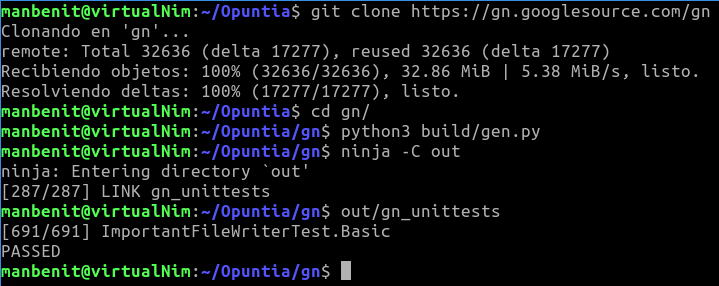
\includegraphics[scale=0.4]{installGn.png}
	\end{center}
\end{frame}

\begin{frame}{Instalación de LLVM}
	\begin{center}
		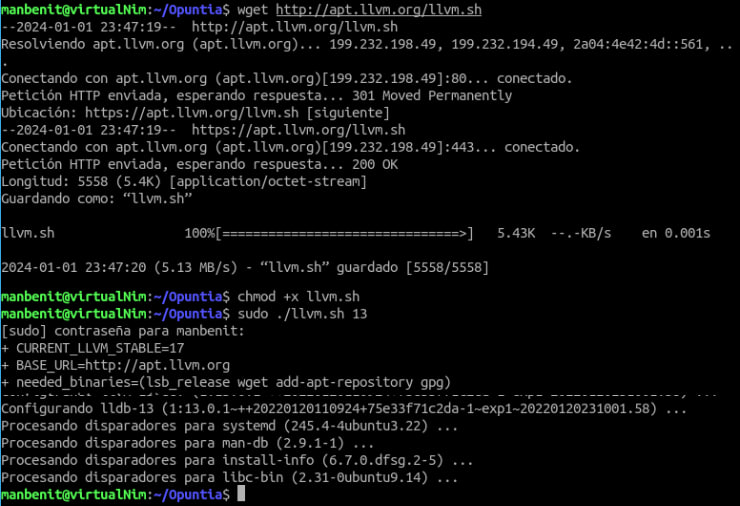
\includegraphics[scale=0.5]{installLlvm.jpg}
	\end{center}
\end{frame}

\begin{frame}{Instalación del \textit{toolchain} para x86}
	\begin{center}
		\ttfamily
		chmod 775 toolchains/scripts/i686-elf-tools.sh
		
		
		
		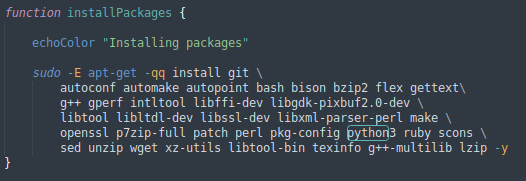
\includegraphics[scale=0.55]{modificarPython.png}
		
		
		
		./toolchains/scripts/i686-elf-tools.sh
	\end{center}
\end{frame}

\begin{frame}{Instalación del \textit{toolchain} para x86}
	\begin{center}
		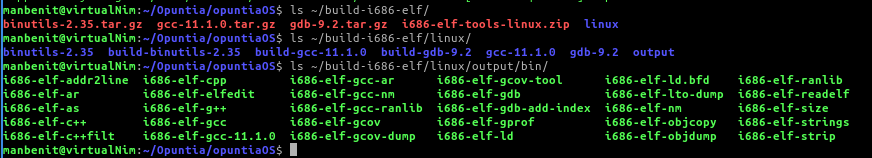
\includegraphics[scale=0.35]{toolchainx86_res.png}
		
		
		
		\ttfamily
		export PATH=\$PATH:<directorio\_de\_contrucción>/linux/output/bin
	\end{center}
\end{frame}


\begin{frame}{Instalación de \textit{toolchain} para ARM}
	\begin{center}
		\ttfamily
		chmod 775 toolchains/scripts/arm-none-eabi-tools.sh
		
		
		
		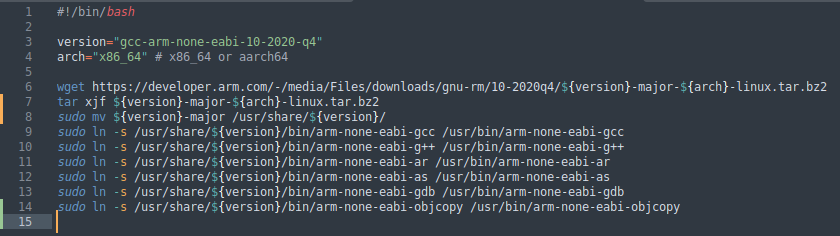
\includegraphics[scale=0.35]{modifArmSsh.png}
		
		
		
		./toolchains/scripts/arm-none-eabi-tools.sh
	\end{center}
\end{frame}

\begin{frame}{Instalación del \textit{toolchain} para ARM}
	\begin{center}
		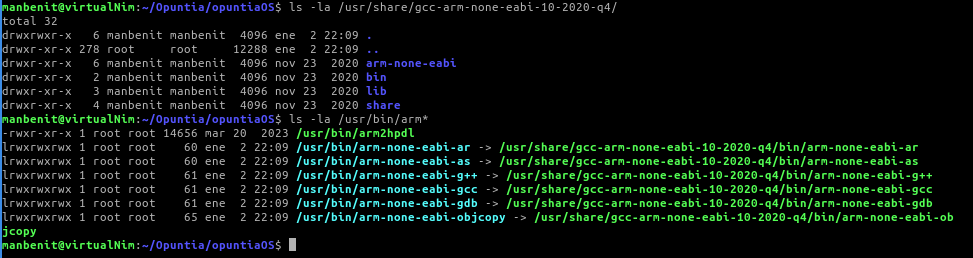
\includegraphics[scale=0.3]{toolchainArm_res.png}
	\end{center}
\end{frame}



%\section{Contrucción}

\section{Análisis}
\begin{frame}{}
	
\end{frame}

\begin{frame}{Implementación del \textit{bootloader}}
	Lo primero de lo que es posible percatarse al analizar la implementación del \textit{bootloader} es que la estructura de carpetas y archivos es distinta para \texttt{ARM} y \texttt{x86}.
	\begin{center}
		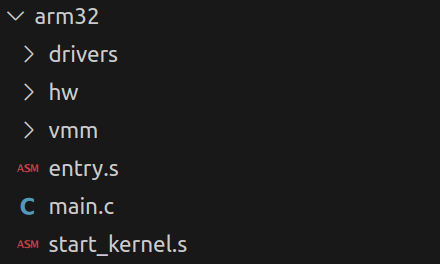
\includegraphics[scale=0.3]{estrucDir_ARM.png}
		\hspace{0.5cm}
		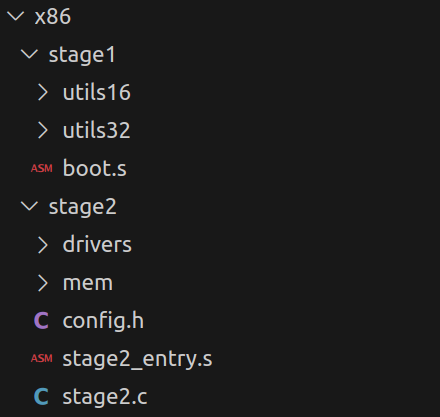
\includegraphics[scale=0.3]{estrucDir_x86.png}
	\end{center}
\end{frame}

\begin{frame}{Implementación del \textit{bootloader}}
	En el caso de \texttt{OpuntiaOS} para \texttt{x86}, se manejan 2 archivos de etapa para el arranque del sistema en lugar de 1, es decir, no se generará el archivo \texttt{stage2\_eltorito}, si no que se generarán 2 archivos de carga de \textit{kernel}.
	\begin{center}
		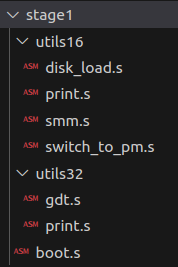
\includegraphics[scale=0.3]{x86_stage1_code.png}
		\hspace{0.5cm}
		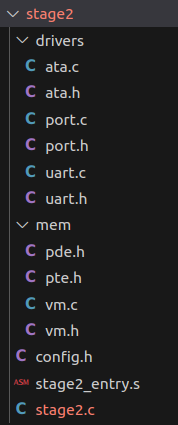
\includegraphics[scale=0.3]{x86_stage2_code.png}
	\end{center}
\end{frame}

\begin{frame}{Implementación del \textit{bootloader}}
	La primera etapa de carga contiene solo código ensamblador, es to es porque \texttt{stage1} se carga desde la BIOS y es la encargado de realizar la primera carga del \textit{kernel}, se puede decir que el archivo más importante es \texttt{boot.s}, similar a los \textit{kernel} compilados en el curso.
\end{frame}


\begin{frame}{Implementación del \textit{bootloader}}
	En el caso de \texttt{OpuntiaOS} para \texttt{ARM}, el \textit{bootloader} trabaja en 2 etapas, la primera en modo supervisor, que se encarga de acceder a los recursos del sistema y poder ejecutar el \textit{kernel} del sistema y la de modo usuario, donde se restringe el acceso a \textit{hardware}.
	\begin{center}
		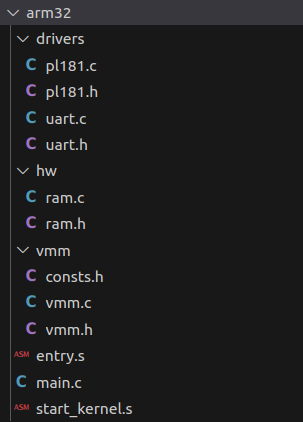
\includegraphics[scale=0.25]{arm_boot_code.png}
	\end{center}
\end{frame}

\begin{frame}{Implementación del \textit{bootloader}}
	La primera etapa de carga contiene solo código ensamblador, esto es porque \texttt{stage1} se carga desde la BIOS y es la encargado de realizar la primera carga del \textit{kernel}, se puede decir que el archivo más importante es \texttt{boot.s}, similar a los \textit{kernel} compilados en el curso.
\end{frame}

\begin{frame}{Implementación del \textit{bootloader}}
	La implementación del \textit{bootloader} de ambas arquitecturas utiliza, en común, los archivos del directorio \texttt{libboot}, que contiene las estructuras de datos y algunas implementaciones para hacer la validación del sistema (firma, seguridad, sistema de archivos \texttt{ext2}, etc.) y que éste arranque de forma correcta y segura.
\end{frame}

\begin{frame}{Implementación del \textit{bootloader}}
	\begin{figure}[ht]
		\centering
		\subfloat{
			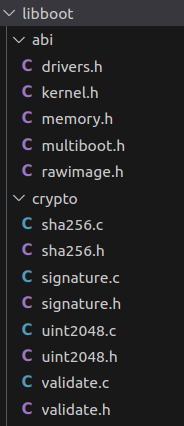
\includegraphics[scale=0.35]{libboot_p1.png}
		}
		\hspace*{1cm}
		\subfloat{
			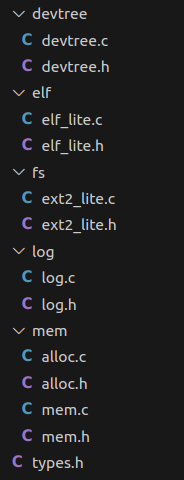
\includegraphics[scale=0.35]{libboot_p2.png}
		}
	\end{figure}
\end{frame}


\begin{frame}{Implementación del \textit{bootloader}}
	Otro directorio que implementan en común las 2 arquitecturas es \texttt{libs}, que contiene, entre otras cosas, manejadores de memoria, definiciones para funcionamiento de la interfás gráfica y las definiciones de funciones para lenguaje \texttt{C}, tales como \texttt{malloc, execve, fork}, etc.
\end{frame}

\begin{frame}{Implementación del \textit{bootloader}}
	\begin{figure}[ht]
		\centering
		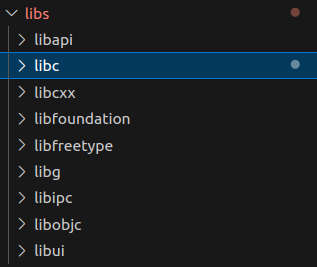
\includegraphics[scale=0.5]{libs.png}
	\end{figure}
\end{frame}



\section{Comparativa}
\begin{frame}{Similitud entre ambas arquitecturas}
	\begin{itemize} \setlength\itemsep{0pt}
		\item \textbf{Inicialización del hardware}: Detectar y configurar la memoria, el CPU, los dispositivos de almacenamiento y otros componentes del sistema.
		
		\item \textbf{Carga del sistema operativo}: Buscar y cargar el \textit{kernel} del sistema operativo en la memoria.
		
		\item \textbf{Transferencia de control}: Transferir el control al \textit{kernel} del sistema operativo para que se inicie el sistema.
		
		\item \textbf{Fase de arranque temprano}: Se ejecuta en \textbf{modo real} en \texttt{x86} y en \textbf{modo supervisor} en \texttt{ARM}. 
		
		En esta fase se hace una inicialización básica del \textit{hardware} y carga el \textit{kernel} del \textit{bootloader}.
		
		\item \textbf{Fase de arranque tardío}: Se ejecuta en \textbf{modo protegido} en \texttt{x86} y en \textbf{modo usuario} en \texttt{ARM}. 
	\end{itemize}
\end{frame}


\begin{frame}{Diferencias entre ambas arquitecturas}
	\centering
	\scalebox{0.85}{
		\begin{tabular}{|>{\columncolor[HTML]{ECF4FF}}c |c|c|}
			\hline
			\multicolumn{1}{|l|}{\cellcolor[HTML]{000000}} & \cellcolor[HTML]{68CBD0}\textbf{x86} & \cellcolor[HTML]{68CBD0}\textbf{ARM}                                                    \\ \hline
			\textbf{Instrucciones}                         & Complejas, de 16 y 32 bits           & Reducidas, de 32 bits                                                                     \\ \hline
			\textbf{Modo de arranque}                      & En modo real                         & En modo supervisor                                                                      \\ \hline
			\textbf{Acceso a hardware}                     & Tiene acceso directo                 & \begin{tabular}[c]{@{}c@{}}Utiliza interfaces del \\ firmware del sistema\end{tabular} \\ \hline
			\textit{\textbf{Firmware}}                     & Utiliza BIOS                         & Utiliza U-Boot o UEFI                                                                   \\ \hline
			\textbf{Herramientas}                          & GRUB y LILO                          & U-Boot y UEFI                                                                           \\ \hline
		\end{tabular}
	}
\end{frame}

\begin{frame}{Diferencias entre ambas arquitecturas}
	Durante el curso de sistemas operativos se abordo el tema del modo real y modo protegido de la arquitectura\texttt{x86}, siendo el primero cuando se tiene acceso directo a rutinas de la BIOS y el \textit{hardware} y el segundo cuando se restringe el acceso a privilegios del sistema usando GDT, IDT y memoria virtual por paginación.
	
	En \texttt{ARM} existen homólogos denominados ``modo supervisor'' y ``modo usuario'', que cumplen una función similar al modo real y protegido, respectivamente.
\end{frame}

\begin{frame}{Diferencias entre ambas arquitecturas: arranque ARM}
	\textbf{Protección}
	
	\begin{itemize} \setlength\itemsep{0pt}
		\item \underline{Modo supervisor}: Permite el acceso a recursos sensibles como memoria, dispositivos de E/S e instrucciones privilegiadas. Se utiliza para ejecutar el \textit{kernel}, controladores de dispositivos y otras tareas críticas del sistema.
		
		\item \underline{Modo usuario}: Limita el acceso a recursos del sistema y solo permite ejecutar instrucciones no privilegiadas. Se usa para ejecutar aplicaciones de usuario, esto protege el sistema operativo y el \textit{hardware} de posibles errores o acciones maliciosas.
	\end{itemize}
\end{frame}

\begin{frame}{Diferencias entre ambas arquitecturas: arranque ARM}
	\textbf{Aislamiento}
	
	\begin{itemize} \setlength\itemsep{0pt}
		\item \underline{Modo supervisor}: Ofrece un entorno seguro para ejecutar el sistema operativo y las tareas críticas del sistema, sin interferencias de las aplicaciones de usuario.
		
		\item \underline{Modo usuario}: Proporciona un entorno aislado para ejecutar aplicaciones de usuario, evitando que puedan acceder a recursos del sistema que no necesitan.
	\end{itemize}
\end{frame}

\begin{frame}{Diferencias entre ambas arquitecturas: arranque ARM}
	\textbf{Rendimiento}
	
	\begin{itemize} \setlength\itemsep{0pt}
		\item \underline{Modo supervisor}: Permite un mayor rendimiento al ejecutar código privilegiado que necesita acceso directo al \textit{hardware}.
		
		\item \underline{Modo usuario}: Permite un uso más eficiente de la memoria al ejecutar código no privilegiado en un espacio de memoria separado.
	\end{itemize}
\end{frame}

\begin{frame}{Diferencias entre ambas arquitecturas}
	\centering
	\scalebox{0.85}{
		\begin{tabular}{|
				>{\columncolor[HTML]{ECF4FF}}c |c|c|}
			\hline
			\multicolumn{1}{|l|}{\cellcolor[HTML]{000000}}                                 & \cellcolor[HTML]{68CBD0}\textbf{Modo real} & \cellcolor[HTML]{68CBD0}\textbf{Modo supervisor}                            \\ \hline
			\textbf{Nivel de privilegios}                                                  & Bajo                                       & Alto                                                                        \\ \hline
			\textbf{Acceso a memoria}                                                      & Segmentado                                 & Completo                                                                    \\ \hline
			\textbf{\begin{tabular}[c]{@{}c@{}}Acceso a \\ dispositivos E/S\end{tabular}}  & Limitado                                   & Completo                                                                    \\ \hline
			\textbf{\begin{tabular}[c]{@{}c@{}}Ejecución de \\ instrucciones\end{tabular}} & No privilegiadas                           & \begin{tabular}[c]{@{}c@{}}Privilegiadas y \\ no privilegiadas\end{tabular} \\ \hline
		\end{tabular}
	}
\end{frame}

\begin{frame}{Diferencias entre ambas arquitecturas}
	\centering
	\scalebox{0.85}{
	\begin{tabular}{|
				>{\columncolor[HTML]{ECF4FF}}c |c|c|}
			\hline
			\multicolumn{1}{|l|}{\cellcolor[HTML]{000000}}                                 & \cellcolor[HTML]{68CBD0}\textbf{Modo protegido}                                & \cellcolor[HTML]{68CBD0}\textbf{Modo usuario}                                \\ \hline
			\textbf{Nivel de privilegios}                                                  & Alto                                                                           & Bajo                                                                         \\ \hline
			\textbf{Acceso a memoria}                                                      & \begin{tabular}[c]{@{}c@{}}Segmentado y \\ paginado\end{tabular}               & \begin{tabular}[c]{@{}c@{}}Limitado por \\ el segmento\end{tabular}          \\ \hline
			\textbf{\begin{tabular}[c]{@{}c@{}}Acceso a \\ dispositivos E/S\end{tabular}}  & \begin{tabular}[c]{@{}c@{}}Controlado por el \\ sistema operativo\end{tabular} & \begin{tabular}[c]{@{}c@{}}Limitado por el \\ sistema operativo\end{tabular} \\ \hline
			\textbf{\begin{tabular}[c]{@{}c@{}}Ejecución de \\ instrucciones\end{tabular}} & \begin{tabular}[c]{@{}c@{}}Privilegiadas y \\ no privilegiadas\end{tabular}    & \begin{tabular}[c]{@{}c@{}}No \\ privilegiadas\end{tabular}             \\ \hline
		\end{tabular}
	}
\end{frame}

\begin{frame}{Diferencias entre ambas arquitecturas: Arranque de \textit{bootloader}}
	\centering
	\resizebox{\textwidth}{!}{
		\begin{tabular}{|c|cc|}
			\hline
			\rowcolor[HTML]{68CBD0} 
			\multicolumn{1}{|l|}{\cellcolor[HTML]{000000}}                                & \multicolumn{1}{c|}{\cellcolor[HTML]{68CBD0}\textbf{x86}}                                                                                                                    & \textbf{ARM}                                                                                                                                                   \\ \hline
			\cellcolor[HTML]{ECF4FF}\textbf{Ubicación}                                    & \multicolumn{1}{c|}{\begin{tabular}[c]{@{}c@{}}MBR del disco \\ de arranque\end{tabular}}                                                                                    & \begin{tabular}[c]{@{}c@{}}Disco de arranque\\ (ej: tarjeta SD)\end{tabular}                                                                                   \\ \hline
			\cellcolor[HTML]{ECF4FF}\textbf{Modo de ejecución}                            & \multicolumn{1}{c|}{Modo real}                                                                                                                                               & Modo supervisor                                                                                                                                                \\ \hline
			\cellcolor[HTML]{ECF4FF}\textbf{Funciones}                                    & \multicolumn{1}{c|}{\begin{tabular}[c]{@{}c@{}}- Carga el \textit{kernel} del sistema operativo. \\ - Transfiere el control al \textit{kernel}. \\ - Ofrece un menú de arranque.\end{tabular}} & \begin{tabular}[c]{@{}c@{}}- Carga el \textit{kernel} del sistema operativo. \\ - Transfiere el control al \textit{kernel}. \\ - Puede ofrecer un menú de arranque.\end{tabular} \\ \hline
			\textbf{\begin{tabular}[c]{@{}c@{}}Diferencias más\\ relevantes\end{tabular}} & \multicolumn{1}{c|}{\begin{tabular}[c]{@{}c@{}}- Arranca en modo real. \\ - Código de 16 bits. \\ - Acceso directo al \textit{hardware}.\end{tabular}}                                & \begin{tabular}[c]{@{}c@{}}- Arranca en modo supervisor. \\ - Código de 32 bits (o 64 bits). \\ - Usa interfaces del \textit{firmware}.\end{tabular}                    \\ \hline
			\textbf{Similitudes}                                                          & \multicolumn{2}{c|}{\begin{tabular}[c]{@{}c@{}}- Carga el \textit{kernel} del sistema operativo. \\ - Transfiere el control al \textit{kernel}. \\ - Ofrece opciones de configuración.\end{tabular}}                                                                                                                                                            \\ \hline
			\cellcolor[HTML]{ECF4FF}\textbf{Ejemplos}                                     & \multicolumn{1}{c|}{GRUB, LILO}                                                                                                                                              & U-Boot, UEFI                                                                                                                                                   \\ \hline
		\end{tabular}
	}
\end{frame}



\section{Temas vistos en clase}
\begin{frame}
	El código fuente del \textit{kernel} de \texttt{OpuntiaOS} se encuentra en el directorio \texttt{kernel} y está dividido en 2 directorios, \texttt{include} y \texttt{kernel}.
	
	Ambos directorios tienen, prácticamente, la misma estructura, pero el directorio \texttt{include} contiene archivo \texttt{.h} para definir las funciones y constantes necesarias para la compilación del \textit{kernel}, mientras que \texttt{kernel} contiene las implementaciones de estas cabeceras.
\end{frame}

\begin{frame}
	\begin{figure}[ht]
		\centering
		\subfloat{
			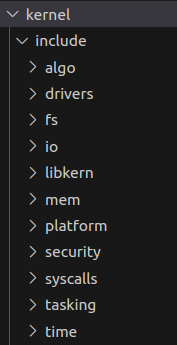
\includegraphics[scale=0.5]{kernel_code_include.png}
		}
		\hspace{3cm}
		\subfloat{
			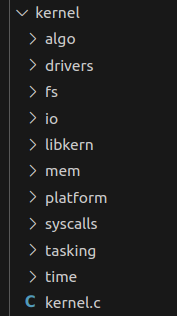
\includegraphics[scale=0.5]{kernel_code_kernel.png}
		}
	\end{figure}
\end{frame}


\begin{frame}
	Una particularidad de esta estructura de carpetas es el directorio \texttt{platform}, el cual contiene las definiciones e implementaciones, respectivamente, que corresponden a cada una de las arquitecturas que soporta \texttt{OpuntiaOS}.
	
	A continuación se empatará el código visto en el curso con el contenido del código de \texttt{OpuntiaOS} siguiendo el orden del proyecto de James Molloy.
\end{frame}


\begin{frame}{Relación James Molloy: Génesis}
	Archivos de Molloy: \texttt{boot.s, link.ld}.
	
	Para x86
	\begin{itemize} \setlength\itemsep{0pt} \footnotesize
		\item \texttt{build/boot/x86/boot\_link.ld}: El programa de carga se coloca en la dirección \texttt{0x1000}.
		\item \texttt{boot/x86/stage1/boot.s}: Carga del kernel.
		\item \texttt{boot/x86/stage2/stage2\_entry.s}: Inicialización de las estructuras del kernel.
	\end{itemize}
	
	NOTA: El archivo \texttt{boot/x86\_64/prekernel/mboot1.S} contiene una estructura mucho más similar al ensamblador proporcionado en el proyecto de Molloy, sin embargo el presente documento contempla la compilación en \texttt{x86} y no en \texttt{x86\_64}.
\end{frame}

\begin{frame}{Relación James Molloy: Génesis}
	Para ARM
	\begin{itemize} \setlength\itemsep{0pt} \footnotesize
		\item \texttt{build/boot/arm32/boot\_link.ld}: El programa de carga se coloca en la dirección \texttt{0x80010000}.
		\item \texttt{boot/arm32/entry.s}: Carga del kernel.
		\item \texttt{boot/arm32/start\_kernel.s}: Inicialización de las estructuras del kernel.
	\end{itemize}
\end{frame}



\begin{frame}{Relación con James Molloy: La pantalla}
	En el código de Molloy se implementan los tipos de dato que se utilizan en todo el proyecto en el archivo \texttt{common.h} y \texttt{common.c}, en \texttt{OpuntiaOS} se usan:
	\begin{itemize} \setlength\itemsep{0pt} \footnotesize
		\item \texttt{boot/libboot/types.h}: Los tipos de dato que utiliza el \textit{bootloader}.
		
		\item \texttt{kernel/include/libkern/types.h}: Los tipos de dato que utiliza el código del \textit{kernel} para poder ser compilado.
		
		\item \texttt{libs/libc/include/sys/types.h}: Los tipos de dato que se utilizan como parte de la implementación, en lenguaje \texttt{C}, del sistema.
	\end{itemize}
	
	Estos archivos son utilizados por ambas arquitecturas.
\end{frame}

\begin{frame}{Relación con James Molloy: La pantalla}
	Luego, Molloy implementa el manejo de la pantalla con los archivos \texttt{monitor.h} y \texttt{monitor.c}; como \texttt{OpuntiaOS} es un sistema con ambiente gráfico, entonces se implementan los siguientes manejadores de pantalla:
	
	la pantalla tal como se vio en el curso, colocando la dirección de memoria de arranque de pantalla, pero se incluye el manejo de el ambiente gráfico y soporte de ventanas del sistema:
	
\end{frame}

\begin{frame}{Relación con James Molloy: La pantalla}
	\begin{itemize} \setlength\itemsep{0pt} \footnotesize
		\item \textbf{Inicialización y control}: Similar al proyecto en clase, se utiliza la pantalla con sus direcciones de memoria y manipulación de caracteres, se usan las definiciones en
		\texttt{kernel/include/drivers/debug/screen.h}\\
		y las implementaciones en 
		\texttt{kernel/kernel/drivers/debug/screen.c}.
		
		\item \textbf{Interfaz gráfica}: Se define el soporte para la interfaz gráfica del sistema en 
		\texttt{libs/libui/include/libui/Screen.h} y se utiliza en \\
		\texttt{libs/libui/src/Window.cpp}. \\
		Como puede notarse, esta implementación es en \texttt{C++}.
		
		
		\item \textbf{Ventanas del sistema}: Se define el manejo de ventanas en el archivo \texttt{userland/servers/window\_server/src/devices/Screen.h}, que se implementa en \texttt{userland/servers/window\_server/src/devices/Screen.cpp}, siendo desarrollado en \texttt{C++} y usándose en varios archivos dentro de\\ \texttt{userland/servers/window\_server/src/Components}.
	\end{itemize}
\end{frame}


\begin{frame}{Relación con James Molloy: GDT e IDT}
	Archivos de Molloy: \texttt{gdt.s, interrupt.s, descriptor\_tables.h, descriptor\_tables.c, isr.h, isr.c}.
	
	Para x86:
	\begin{itemize} \setlength\itemsep{0pt} \footnotesize
		\item Ensambladores
		\begin{itemize} \setlength\itemsep{0pt}
			\item \texttt{boot/x86/stage1/utils32/gdt.s}
			\item \texttt{kernel/kernel/platform/x86/i386/interrupts/interrupts.s}
		\end{itemize}	
		
		\item Descriptor de la GDT
		\begin{itemize} \setlength\itemsep{0pt}
			\item \texttt{kernel/include/platform/x86/gdt.h}
			\item \texttt{kernel/kernel/platform/x86/gdt.c}
		\end{itemize}	
		
		\item Descriptor de la IDT
		\begin{itemize} \setlength\itemsep{0pt}
			\item \texttt{kernel/include/platform/x86/idt.h}
			\item \texttt{kernel/kernel/platform/x86/interrupts/idt.c}
		\end{itemize}
		
	\end{itemize}
\end{frame}


\begin{frame}{Relación con James Molloy: GDT e IDT}
	\begin{itemize} \setlength\itemsep{0pt} \footnotesize
			\item Parte donde se inicia la GDT e IDT
		\begin{itemize} \setlength\itemsep{0pt}
			\item \texttt{kernel/include/platform/x86/init.h}
			\item \texttt{kernel/kernel/platform/x86/init.c}
		\end{itemize}	
		
		\item Manejador de IRQ
		\begin{itemize} \setlength\itemsep{0pt}
			\item \texttt{kernel/include/platform/x86/irq\_handler.h}
			\item \texttt{kernel/kernel/platform/x86/interrupts/irq\_handler.c}
		\end{itemize}	
		
		\item Rutinas de interrupciones (ISR)
		\begin{itemize} \setlength\itemsep{0pt}
			\item \texttt{kernel/include/platform/x86/isr\_handler.h}
			\item \texttt{kernel/kernel/platform/x86/interrupts/isr\_handler.c}
		\end{itemize}	
	\end{itemize}
\end{frame}


\begin{frame}{Relación con James Molloy: GDT e IDT}
	La arquitectura ARM no utiliza una GDT ni una IDT de la misma manera que lo hace la x86.
	
	ARM utiliza un modelo de segmentación de memoria plano (\textit{Flat Memory Model}), lo que significa que no hay segmentos de memoria separados como en x86. En lugar de la IDT, ARM utiliza vectores de interrupción y excepción.
	
\end{frame}



\begin{frame}{Relación con James Molloy: GDT e IDT}
	Para ARM:
	\begin{itemize} \setlength\itemsep{0pt} \footnotesize
		\item Ensambladores
		\begin{itemize} \setlength\itemsep{0pt}
			\item \texttt{kernel/kernel/platform/arm32/interrupts/interrupts.s}
		\end{itemize}
		
		\item Descriptor de la tabla genérica de interrupciones
		\begin{itemize} \setlength\itemsep{0pt}
			\item \texttt{kernel/include/drivers/irq/arm/gicv2.h}
			\item \texttt{kernel/kernel/drivers/irq/arm/gicv2.c}
		\end{itemize}
		
		\item Configuración de interrupciones y excepciones
		\begin{itemize} \setlength\itemsep{0pt}
			\item \texttt{kernel/include/platform/arm32/interrupts.h}
			\item \texttt{kernel/kernel/platform/arm32/interrupts/handlers.c}
		\end{itemize}
		
		\item Parte del código donde se inicia el controlador genérico de interrupciones (GIC) y las interrupciones.
		\begin{itemize} \setlength\itemsep{0pt}
			\item \texttt{kernel/include/platform/arm32/init.h}
			\item \texttt{kernel/kernel/platform/arm32/init.c}
		\end{itemize}	
	\end{itemize}
\end{frame}


\begin{frame}{Relación con James Molloy: IRQ y PIT}
	Archivos de Molloy: \texttt{timer.h, timer.c}.
	
	La PIT)es un componente se utiliza para generar interrupciones periódicas, como las interrupciones del sistema operativo que pueden ser usadas para mantener el tiempo del sistema, gestionar tareas programadas, etc.
	
	En la arquitectura ARM no hay un PIT, si no temporizadores específicos que son parte del diseño del sistema embebido o del SoC, que pueden variar entre diferentes dispositivos.
\end{frame}

\begin{frame}{Relación con James Molloy: IRQ y PIT}
	Para ambas arquitecturas se implementa un Administrador principal de \textit{ticks}:\\
	\texttt{kernel/include/time/time\_manager.h} \\
	\texttt{kernel/kernel/time/time\_manager.c}
\end{frame}

\begin{frame}{Relación con James Molloy: IRQ y PIT}
	Para x86
	\begin{itemize} \setlength\itemsep{0pt} \footnotesize
		\item \texttt{kernel/include/drivers/timer/x86/pit.h}
		\item \texttt{kernel/kernel/drivers/timer/x86/pit.c}
		
	\end{itemize}
	
	Para ARM:
	En el caso de OpuntiaOS, se implementa un temporizador enfocado en el temporizador SP804
	\begin{itemize} \setlength\itemsep{0pt} \footnotesize
		\item \texttt{kernel/kernel/drivers/timer/arm/sp804.c}
		\item \texttt{kernel/include/drivers/timer/arm/sp804.h}
	\end{itemize}
\end{frame}


\begin{frame}{Relación con James Molloy: Paginación}
	Archivos de Molloy: \texttt{paging.h, paging.c, kheap.h, kheap.c}.
	
	
	Se usa el \textit{heap} para los archivos en \texttt{kernel/kernel/io}.
	
	\begin{itemize} \setlength\itemsep{0pt} \footnotesize
		\item Definición del \textit{heap} y su control
		\begin{itemize} \setlength\itemsep{0pt}
			\item \texttt{kernel/include/mem/kmalloc.h}
			\item \texttt{kernel/kernel/mem/kmalloc.c}
		\end{itemize}
		
		\item Gestión de la memoria virtual
		\begin{itemize} \setlength\itemsep{0pt} \footnotesize
			\item \texttt{kernel/include/mem/vmm.h}
			\item \texttt{kernel/kernel/mem/vmm.c}
		\end{itemize}
		
	\end{itemize}
	
	Se utiliza el mismo manejo de memoria para ambas arquitecturas.
\end{frame}


\begin{frame}{Relación con James Molloy: VFS}
	Archivos de Molloy: \texttt{fs.h, fs.c, initrd.h, initrd.c, multiboot.h}.
	
	Se maneja el mismo sistema de archivos para ambas arquitecturas, en este caso, \texttt{ext2}
	\begin{itemize} \setlength\itemsep{0pt}\footnotesize
		\item Creación del \textit{ramdisk}
		\begin{itemize} \setlength\itemsep{0pt}
			\item \texttt{kernel/include/drivers/storage/ramdisk.h}
			\item \texttt{kernel/kernel/drivers/storage/ramdisk.c}
		\end{itemize}
	\end{itemize}
\end{frame}

\begin{frame}{Relación con James Molloy: VFS}
	\begin{itemize} \setlength\itemsep{0pt}\footnotesize
		\item Definición del sistema de archivos virtual
		\begin{itemize} \setlength\itemsep{0pt}
			\item \texttt{kernel/kernel/fs/vfs.h}
			\item \texttt{kernel/include/fs/vfs.c}
		\end{itemize}
	
		\item Definición del sistema de archivos \texttt{ext2}, aquí se encuentra definido el superbloque.
		\begin{itemize} \setlength\itemsep{0pt}
			\item \texttt{kernel/include/fs/ext2/ext2.h}
			\item \texttt{kernel/kernel/fs/ext2/ext2.c}
		\end{itemize}
	\end{itemize}
\end{frame}


\begin{frame}{Relación con James Molloy: Multitarea}
	Archivos de Molloy: \texttt{process.s, task.h, task.c}.
	
	En ambas arquitecturas se tiene la implementación común de tareas:
	\begin{itemize} \setlength\itemsep{0pt}
		\item \texttt{kernel/include/tasking/tasking.h}
		\item \texttt{kernel/kernel/tasking/tasking.c}
	\end{itemize}
	
	Sin embargo, cada una tiene su propia implementación particular.
\end{frame}

\begin{frame}{Relación con James Molloy: Multitarea}
	Para x86:
	\begin{itemize} \setlength\itemsep{0pt}
		\item implementación del TSS
		\begin{itemize} \setlength\itemsep{0pt}
			\item \texttt{kernel/include/platform/x86/tasking/tss.h}
			\item \texttt{kernel/kernel/platform/x86/tasking/tss.c}
		\end{itemize}
	\end{itemize}
	
	Para ARM:\\
	La implementación se divide en varios archivos \texttt{.c} y ensambladores, debido a que no se realiza de la misma manera que en \texttt{x86}, se encuentra en los archivos dentro de
	\texttt{kernel/kernel/platform/arm32/tasking}:
\end{frame}

\begin{frame}{Relación con James Molloy: Multitarea}
	\begin{itemize} \setlength\itemsep{0pt} \footnotesize
		\item \textbf{Interrupciones y Excepciones}: En \texttt{x86} la interrupción de temporizador (\textit{timer interrupt}) es crucial para implementar programación de tiempo compartido, mientras que en \texttt{ARM} define modos de operación (usuario, supervisor y otros) que se utilizan para gestionar niveles de privilegio.
		
		\item \textbf{Cambios de Contexto}: En \texttt{x86} el SO mantiene un contexto de registro y estado para cada tarea, luego cuando se produce una interrupción de temporizador solicitud de cambio, se guarda el contexto actual y se carga el contexto de la nueva tarea.
		
		Por otro lado, en \texttt{ARM} se mantiene un contexto de registro y estado para cada tarea en el espacio de memoria específico de cada tarea, luego cambiar entre tareas implica guardar y restaurar el contexto relevante.
		
		\item \textbf{Despacho de Tareas}: En \texttt{x86} se gestionan las prioridades de las tareas y se asigna tiempo de procesador según las políticas de planificación del SO, mientras que en \texttt{ARM} tanto la asignación de tiempo de procesador como la gestión de prioridades son parte de la lógica del planificador.
	\end{itemize}
\end{frame}

\begin{frame}{Relación con James Molloy: Modo usuario}
	Archivos de Molloy: \texttt{syscall.h, syscall.c}.
	
	En el caso de \texttt{OpuntiaOS}, las llamadas al sistema se definen por medio del archivo \texttt{}, a manera de tabla de llamadas al sistema (como el \textit{kernel} de Linux).
	
	Luego se tienen los siguientes archivos relevantes:
	\begin{itemize} \setlength\itemsep{0pt} \footnotesize
		\item \texttt{kernel/include/libkern/bits/syscalls.h}: Definición del número de llamada al sistema para cada arquitectura.
		
		\item \texttt{kernel/include/syscalls/handlers.h}: Definición de las macros de funciones para implementar las llamadas y nombres de dichas funciones.
		
		\begin{itemize} \setlength\itemsep{0pt}
			\item \texttt{kernel/kernel/syscalls/handler.c}: Enlace del número de llamada con su macro de implementación, similar al archivo \texttt{.tbl} del \textit{kernel} de Linux.
		\end{itemize}
	\end{itemize}
\end{frame}




\section{Estructuras de datos}
\begin{frame}{Adminsitrador de procesos}
	\texttt{kernel/include/tasking/proc.h}
	
	\texttt{kernel/include/tasking/thread.h}
	
	\texttt{kernel/include/libkern/bits/signal.h}
\end{frame}


\begin{frame}{Planificador}
	\texttt{kernel/include/tasking/bits/sched.h}
	
	\texttt{kernel/include/platform/x86/i386/tasking/trapframe.h}
	
	\texttt{kernel/include/platform/arm32/tasking/trapframe.h}
	
	\texttt{kernel/include/platform/x86/i386/tasking/context.h}
	
	\texttt{kernel/include/platform/arm32/tasking/context.h}
\end{frame}


\begin{frame}{Administrador de memoria}
	\texttt{kernel/include/platform/generic/vmm/mapping\_table.h}
	
	\texttt{kernel/include/mem/memzone.h}
	
	\texttt{kernel/include/mem/vmm.h}
	
	\texttt{kernel/include/mem/vm\_address\_space.h}
	
	\texttt{kernel/include/mem/bits/vm.h}
\end{frame}


\begin{frame}{Sistema de archivos}
	\texttt{kernel/include/fs/vfs.h}
	
	\texttt{boot/libboot/fs/ext2\_lite.h}
\end{frame}


\begin{frame}{Controladores de dispositivo}
	\texttt{kernel/include/drivers/bits/device.h}
	
	\texttt{kernel/include/drivers/devtree.h}
\end{frame}
